\documentclass[a4paper,12pt]{article}

% Configuração de idioma e codificação
\usepackage[utf8]{inputenc}
\usepackage[T1]{fontenc}
\usepackage[brazil]{babel}

% Layout da página
\usepackage[a4paper, margin=0.8in]{geometry}
\usepackage{setspace}
\setstretch{1.5} % Espaçamento entre linhas

% Fontes e formatação
\usepackage{kpfonts}
\usepackage{amsmath, bm} % Pacotes matemáticos
\usepackage{graphicx} % Inclusão de imagens
\usepackage{caption} % Estilização de legendas
\usepackage{fancyhdr} % Personalização de cabeçalhos e rodapés
\usepackage{titlesec} % Personalização de títulos de seção
\usepackage{xcolor} % Cores para textos e seções
\usepackage{hyperref} % Links clicáveis
\usepackage{background} % Fundo para a página de título
\usepackage{placeins} % Controle de posicionamento de floats (FloatBarrier)
% Ensure the package is loaded correctly for \floatbarrier

\hypersetup{
    colorlinks=true,
    linkcolor=red,
    urlcolor=red,
    citecolor=red
}

% Personalização dos títulos
\titleformat{\section}{\Large\bfseries\color{black}}{\thesection}{1em}{}
\titleformat{\subsection}{\large\bfseries\color{black}}{\thesubsection}{1em}{}

% Cabeçalhos e Rodapés
\pagestyle{fancy}
\fancyhf{}
\fancyhead[R]{
\includegraphics[width=2cm]{ITA.png}} % Logo no topo direito
\fancyhead[L]{\textbf{Instituto Tecnológico de Aeronáutica (ITA)}}
\fancyfoot[L]{Leonardo Peres Dias}
\fancyfoot[R]{\thepage}

% Informações do título
\title{
    \textbf{Inteligência Artificial para Robótica Móvel CT-213}\\
    \Large Instituto Tecnológico de Aeronáutica 

    \textbf{Relatório do Laboratório 8 - Redes Neurais Convolucionais}\\
}
\author{
    Leonardo Peres Dias 
}
\date{\today}

% Configuração do fundo (marca d'água apenas na primeira página)
\backgroundsetup{
    scale=1.5,
    color=black,
    opacity=0.2,
    angle=0,
    position=current page.south,
    vshift=5cm,
    hshift=0cm,
    contents={
\includegraphics[width=8cm]{ITA.png}}
}

% Início do Documento
\begin{document}

% Aplicar o fundo apenas na primeira página
\BgThispage
\maketitle
\thispagestyle{empty} % Sem cabeçalho/rodapé na página de título

%\begin{abstract}
%Este documento apresenta o relatório do Projeto CES-30 - 2024, desenvolvido com base na segunda forma descrita no enunciado do exame. O projeto abrange tarefas de \textbf{mineração de dados} e \textbf{construção de grafos de conhecimento}, com a aplicação de técnicas específicas para análise e solução prática de problemas reais.
%\end{abstract}

\newpage
\NoBgThispage % Desativa a marca d'água para as páginas seguintes

\tableofcontents

\newpage
\NoBgThispage % Desativa a marca d'água para as páginas seguintes

\section{Breve Explicação em Alto Nível da Implementação}

A implementação da rede LeNet-5 foi realizada utilizando a API \texttt{Sequential} do Keras. A arquitetura segue de forma fiel o modelo original proposto por LeCun et al., composto por uma combinação de camadas convolucionais, de pooling e densas. A rede recebe como entrada imagens em escala de cinza com resolução $32 \times 32$.

O modelo é estruturado da seguinte forma:

\begin{itemize}
    \item Uma camada convolucional com 6 filtros $5 \times 5$ e função de ativação tangente hiperbólica (tanh), produzindo saídas de dimensão $28 \times 28 \times 6$.
    \item Uma camada de pooling média (average pooling) com janelas $2 \times 2$ e stride 2, reduzindo a dimensão para $14 \times 14 \times 6$.
    \item Uma segunda camada convolucional com 16 filtros $5 \times 5$ e ativação \texttt{tanh}, resultando em mapas de ativação de tamanho $10 \times 10 \times 16$.
    \item Uma nova camada de pooling média, que reduz a saída para $5 \times 5 \times 16$.
    \item Uma terceira camada convolucional com 120 filtros $5 \times 5$ e ativação \texttt{tanh}, produzindo uma saída de dimensão $1 \times 1 \times 120$.
    \item A saída é achatada (flatten) e conectada a uma camada densa com 84 neurônios e ativação \texttt{tanh}.
    \item Por fim, a rede possui uma camada de saída com 10 neurônios e ativação \texttt{softmax}, adequada para classificação em 10 classes.
\end{itemize}

\newpage

\section{Figuras Comprovando Funcionamento do Código}
\subsection{Evolução do treinamento no \textit{TensorBoard}}
\begin{figure}[htbp]
    \centering
    \begin{tabular}{cc}
        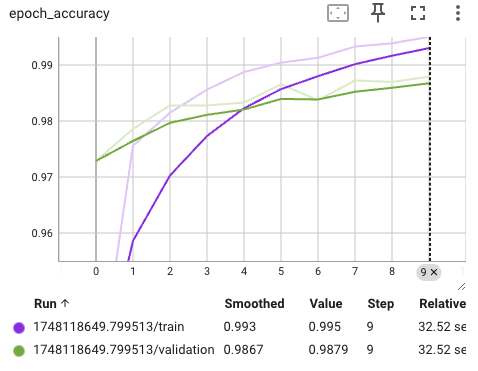
\includegraphics[width=0.45\textwidth]{epoch_accuracy.png} &
        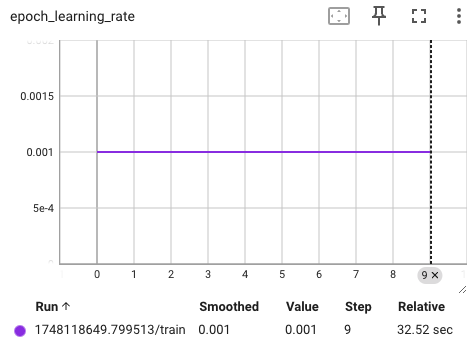
\includegraphics[width=0.45\textwidth]{epoch_learning_rate.png} \\
        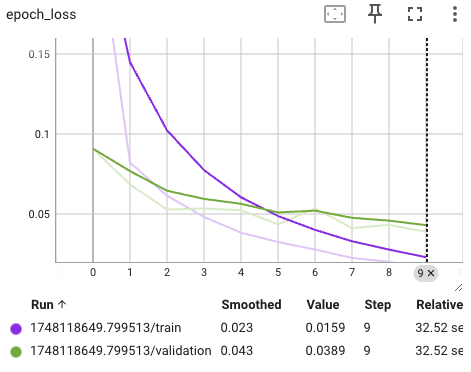
\includegraphics[width=0.45\textwidth]{epoch_loss.png} &
        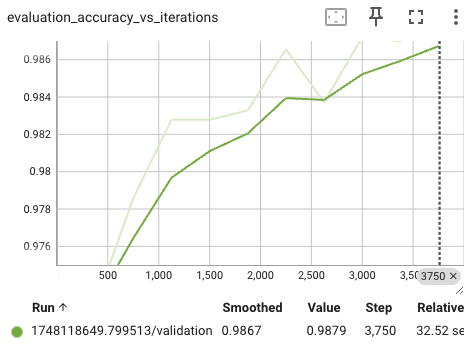
\includegraphics[width=0.45\textwidth]{evaluatoion_acc_vs_iterations.png} \\
        \multicolumn{2}{c}{%
            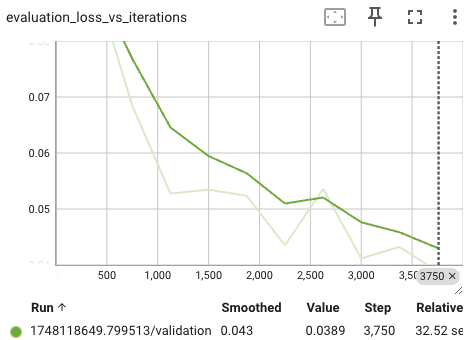
\includegraphics[width=0.45\textwidth]{evaluation_loss_vs_iterations.png}%
        } \\
    \end{tabular}
    \caption{Evolução das métricas de treinamento.}
    \label{fig:images-grid}
\end{figure}

\newpage
\subsection{Avaliação da LeNet-5}

\begin{figure}[htbp]
    \centering
    \begin{minipage}{0.45\textwidth}
        \centering
        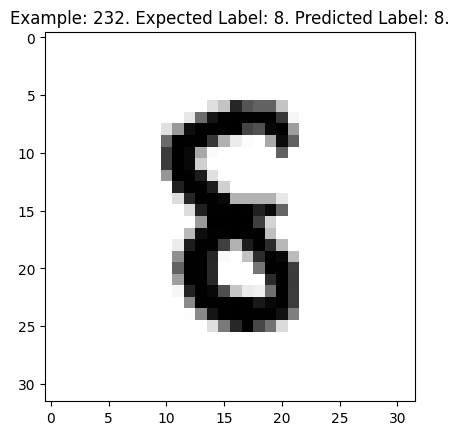
\includegraphics[width=\textwidth]{predicaocerta.png}
        \caption{Predição correta da rede.}
        \label{fig:imagem1}
    \end{minipage}\hfill
    \begin{minipage}{0.45\textwidth}
        \centering
        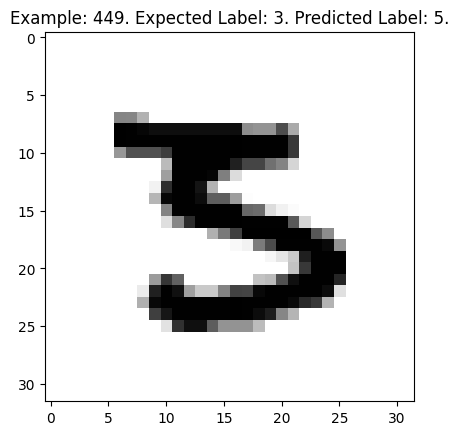
\includegraphics[width=\textwidth]{predicaoerrada.png}
        \caption{Predição errada da rede.}
        \label{fig:imagem2}
    \end{minipage}
\end{figure}

\section{Discussões dos Resultados}

Observa-se na curva de acurácia por época que o modelo apresentou uma evolução consistente durante o treinamento, alcançando aproximadamente 99.5\% de acurácia no conjunto de treino e cerca de 98.8\% no conjunto de validação após 10 épocas. Essa diferença entre treino e validação é pequena, indicando que o modelo generaliza bem para dados não vistos.

A curva de perda (\textit{loss}) de maneira suave tanto para o treino quanto para a validação, refletindo o aprendizado efetivo da rede. A \textit{loss} final de validação estabiliza em torno de 0.039, o que corrobora o bom desempenho do modelo.

O gráfico de taxa de aprendizado confirma que foi utilizada uma taxa fixa de 0.001 durante todas as épocas, sem agendamentos dinâmicos.

Já os gráficos de avaliação por iteração mostram que, conforme o número de iterações aumenta, a acurácia de validação sobe gradualmente, alcançando cerca de 98.7\% ao final do treinamento, enquanto a \textit{loss} de validação apresenta tendência de queda, reforçando a convergêcia do processo de otimização.


Os exemplos apresentados evidenciam tanto a capacidade da rede em reconhecer corretamente os dígitos quanto suas limitações em casos ambíguos. O erro de classificação observado é compreensível, dado que certos dígitos manuscritos podem ter formas semelhantes, o que pode confundir mesmo classificadores robustos como a LeNet-5.


\end{document}